%%
%%  chapter00.tex - Obstacle Detection and Planning for Autonomous Vehicles based on Computer Vision Techniques
%%
%%  Copyright 2014 Néstor Morales <nestor@isaatc.ull.es>
%%
%%  This work is licensed under a Creative Commons Attribution 4.0 International License.
%%

\graphicspath{{./images/chapter00/bmps/}{./images/chapter00/vects/}{./images/chapter00/}}

\chapter{Problem Statement and Previous Work}\label{ch:chapter00}

\section{Problem Statement}\label{ch:chapter00_01}

Computer Vision environment understanding targeted at enabling autonomous operation of a robotic platform has been widely studied over the years, leading to the creation of some prototype vehicles \cite{Maurer1996,Pomerleau1996,Broggi1999} which demonstrated that negotiating moderately complex and dynamic situations in real time was possible, albeit challenging. However, it was only with the development effort driven by the DARPA Challenges \cite{Buehler2007, Buehler2009} that the technology required to provide reliable operation both in off-road and urban scenarios proved to be within reach.
The vehicles that successfully took part to this series of events had to integrate planning and actuation capabilities with a sensing suite capable of coping with harsh environments, heavy traffic and wide temperature ranges, while keeping functional over extended amounts of time. Most competitors relied on high-end active sensors \cite{Urmson2008, Montemerlo2008, Bacha2008, Kammel2008}, with some notable exceptions \cite{Broggi2006, Broggi2010}. 

As we discover when looking up to the available literature (See next section, \ref{ch:chapter00_02}), there are many methods for the detection and tracking of obstacles in complex environments, like this for which Verdino is intended to be working. In this sense, a very first approach is that inspired on the work by \cite{primdahl2005change},  \cite{diego2011video} or \cite{vallespi2012prior} was developed. This is based on the fact that, in an image, a high percentage of the scene represented usually corresponds to static objects. Based on that, it looks quite straightforward to think that, having an image representing an area without obstacles, it is possible to detect the obstacles in an scene by just comparing it with an image being taken in real time. For that, we obtained a dataset with geo-referenced images from a closed urbanization taken at different times of the day. A description of this database, as well as of the algorithm pipeline used for the comparison between images pairs can be found at section \todo{ \ref{XXX} }.

However, such approach suffers from several drawbacks. First, as we just use one image per frame, we are no able to know the exact position of the obstacle in the real world \comment{(Anyway, we think that the output of the algorithm is a good starting point for a classification method)}. Also, the quality of detection is highly tied to the size of the image database, so in big areas we need a huge dataset, with the related space and throughput problems associated to that. If we consider changes due to weather or light conditions, this dataset grows exponentially. Finally, we don't know the direction where an obstacle is going to. These are challenging problems that have been solved using different approaches, until we reached a final solution, described in section \todo { \ref{XXX} }.

To solve that, we first developed a method that tries to isolate just the tracking problem with the use of static monocular cameras. Instead of registering pairs of images, we segment the image with the use of foreground extraction techniques, distinguishing between background and foreground. Using the silhouette of the objects in the foreground (which are mainly non-rigid objects, like pedestrians or animals), we apply a non-rigid point set registration algorithm in order to track the different parts of the body of the obstacles separately. This method, inspired in works like those by \cite{starck2007surface}, or \cite{letouzey2011scene}, can be also used for the completion of the global map of the vehicle, or even for tasks more related to \ac{HMI}. This approach is extensively described in section \todo{ \ref{XXX}}.

However, this method still makes use of a very rudimentary method for the localization of the obstacles (See section \todo{ \ref{XXX-subsection_localization}}), and it is limited to static cameras. For the application proposed, we need the cameras installed on the top of the moving prototype, so we can not use foreground segmentation methods anymore for the detection of the objects in the road. A simple solution for that is stop using monocular vision, and start using stereo vision. In the last years, a high number of advanced algorithms has become viable for autonomous driving applications. The problem is that performing a quantitative and meaningful comparison of their performance level, however, is not an easy task, mainly because of the difficulty of producing ground truth information. Older datasets are small, and either synthetic or taken in controlled environments (\cite{Scharstein2002}), thus effectively limiting their usefulness as indicators of the actual algorithms ability to cope with outdoor scenarios. Due to that, it is needed to compare the performance level of some state-of-the-art stereovision-based 3D mapping algorithms in automotive scenarios. This evaluation methodology and the associated results is shown in section \todo{ \ref{XXX}}. \comment{PREGUNTAR A LA GENTE DEL VISLAB SI ESTA DE ACUERDO CON QUE USE ESTO EN LA TESIS, POR SI LAS MOSCAS}.

\comment{Este párrafo y la sección asociada dependerá de lo que consiga sacar más adelante.}\notsure{
Apart from the full-dense 3D reconstruction methods, we also explore the possibility of using a simpler (and faster) reconstruction based on Stixels, like that described by \cite{badino2009stixel}. In particular, we decided to use the implementation by \cite{benenson2012pedestrian}, due to its fast response (about 100 frames per second). The method, described in section \todo{\ref{XXX}}, compares the stixels obtained between frames and tracks the obstacles along the time. This solves all the problems we had: we can use moving cameras, we can locate the obstacles in the map, and also we are able to know the path followed by them.}

Another approach, which makes use of the dense stereo reconstruction algorithms for which we did the evaluation described above, is inspired in the work by \cite{danescu2012particle}, but also from the voxelized world described in \cite{broggi2013}. The key idea is to simplify the 3d reconstructed world into a grid of voxels, each of these representing a certain volume in the world. In this voxelized world, for each voxel above a given occupancy probability threshold, a set of particles part of a particle filter is assigned. Each particle will have a double function: the first, denoting hypotheses (as in the classical particle filter methods); the second, to be used as segmentation criteria in the segmentation of the world into different obstacles. In this way, we consider that two contiguous voxels belong to different obstacles if their obtained direction and sense diverges. A more detailed explanation of the method is found in \todo{\ref{XXX}}.

At this point, we have an acceptable reconstruction of the surroundings of the vehicle, which includes the localization and tracking of the obstacles in the neighborhood of the cart. But the reconstruction of the environment is not the only challenge that an autonomous vehicle has to deal with. Once that a vehicle has an idea of where it is, and where it wants to go, it also needs to know the best way to reach there and, more important, how to avoid the harmful elements it has previously detected using the methods described. This allows a safe trip, both for the pedestrians, cars, etc. in the road, and for the vehicle itself.
As said, Verdino is intended to travel in pedestrian areas where most of the obstacles are pedestrians, so its behavior must be mainly reactive in order to give priority to the safety of paths against the efficiency of the route. Also, there is not a clear traveling path, like a road. Instead of that, the vehicle will be moving around an unstructured area, so there is not something like a \ac{RNDF} that allows a fast calculation of the paths that the car will use to reach a certain point. Because of that, we must consider two different planning levels:
\begin{itemize}
 \item \textbf{Global Planning:}
 As it is not possible to determine a global trajectory based on a \ac{RNDF}, we must use a method able to deal with changing environments for the calculation of a fast and safe path. The idea is that, having a map of the static obstacles in the environment and with the vehicle properly localized on it \cite{Perea2013mcl}, it will generate a path that will allow reaching this destination as fast as possible. This task, which can be solved easily in static environments using graphs or other similar optimization methods, becomes a little bit more challenging in environments like, for example, a parking lot, in which cars are parking and driving off continuously.
 In section \todo{ \ref{XXX} }, the way in which we solved this problem is described. It is based on the border between classes, which is obtained after training a \ac{MSVM} (See Appendix \todo {\ref{XXX}} for more information), considering each single obstacle as a separate class. Instead of using this border for classification purposes, as it is usual, we take advantage of the fact that it will be the safest and smoother distance to the obstacles. Taking this into account, it makes sense to apply this separation line as our path. Also, the use of a different class for each obstacle allows ensuring that the path is safe enough, even in complicate scenarios, like in pedestrian areas.
 
 \item \textbf{Local Planning:}
 In a lower level, we also need a way to make the vehicle know how to follow the generated path. This problem requires a system able to, several times per second, calculate the best steering angle and speed in order to follow the global plan while avoiding the surrounding obstacles. The method, which is inspired in the work of \cite{chu2012local}, receives as input the current position of the vehicle in the map, its orientation, speed and the steering angle. Also, we provide it with the global plan obtained in the upper level. Finally, a map of the dynamic obstacles in the surrounds of the cart is computed and passed to the algorithm.
 
 This dynamic map can be filled with the information provided by sensors like \acp{LIDAR}, among other sensors. But it can can also be computed with the information extracted from cameras, and this is the connection point with the work described in the first part of this Thesis. The detected obstacles are included in the map, so the vehicle is able to avoid them using the calculated steering angle and speed.
 
 The way in which both this map and the speed/steering angle commands is obtained is described in section \ref{XXX}.
\end{itemize}
 
 The whole pipeline of the application developed for this thesis is shown at figure \ref{fig:cp00_pipeline}. 
 
\begin{figure}[thb]\label{fig:cp00_pipeline}
  \centering
  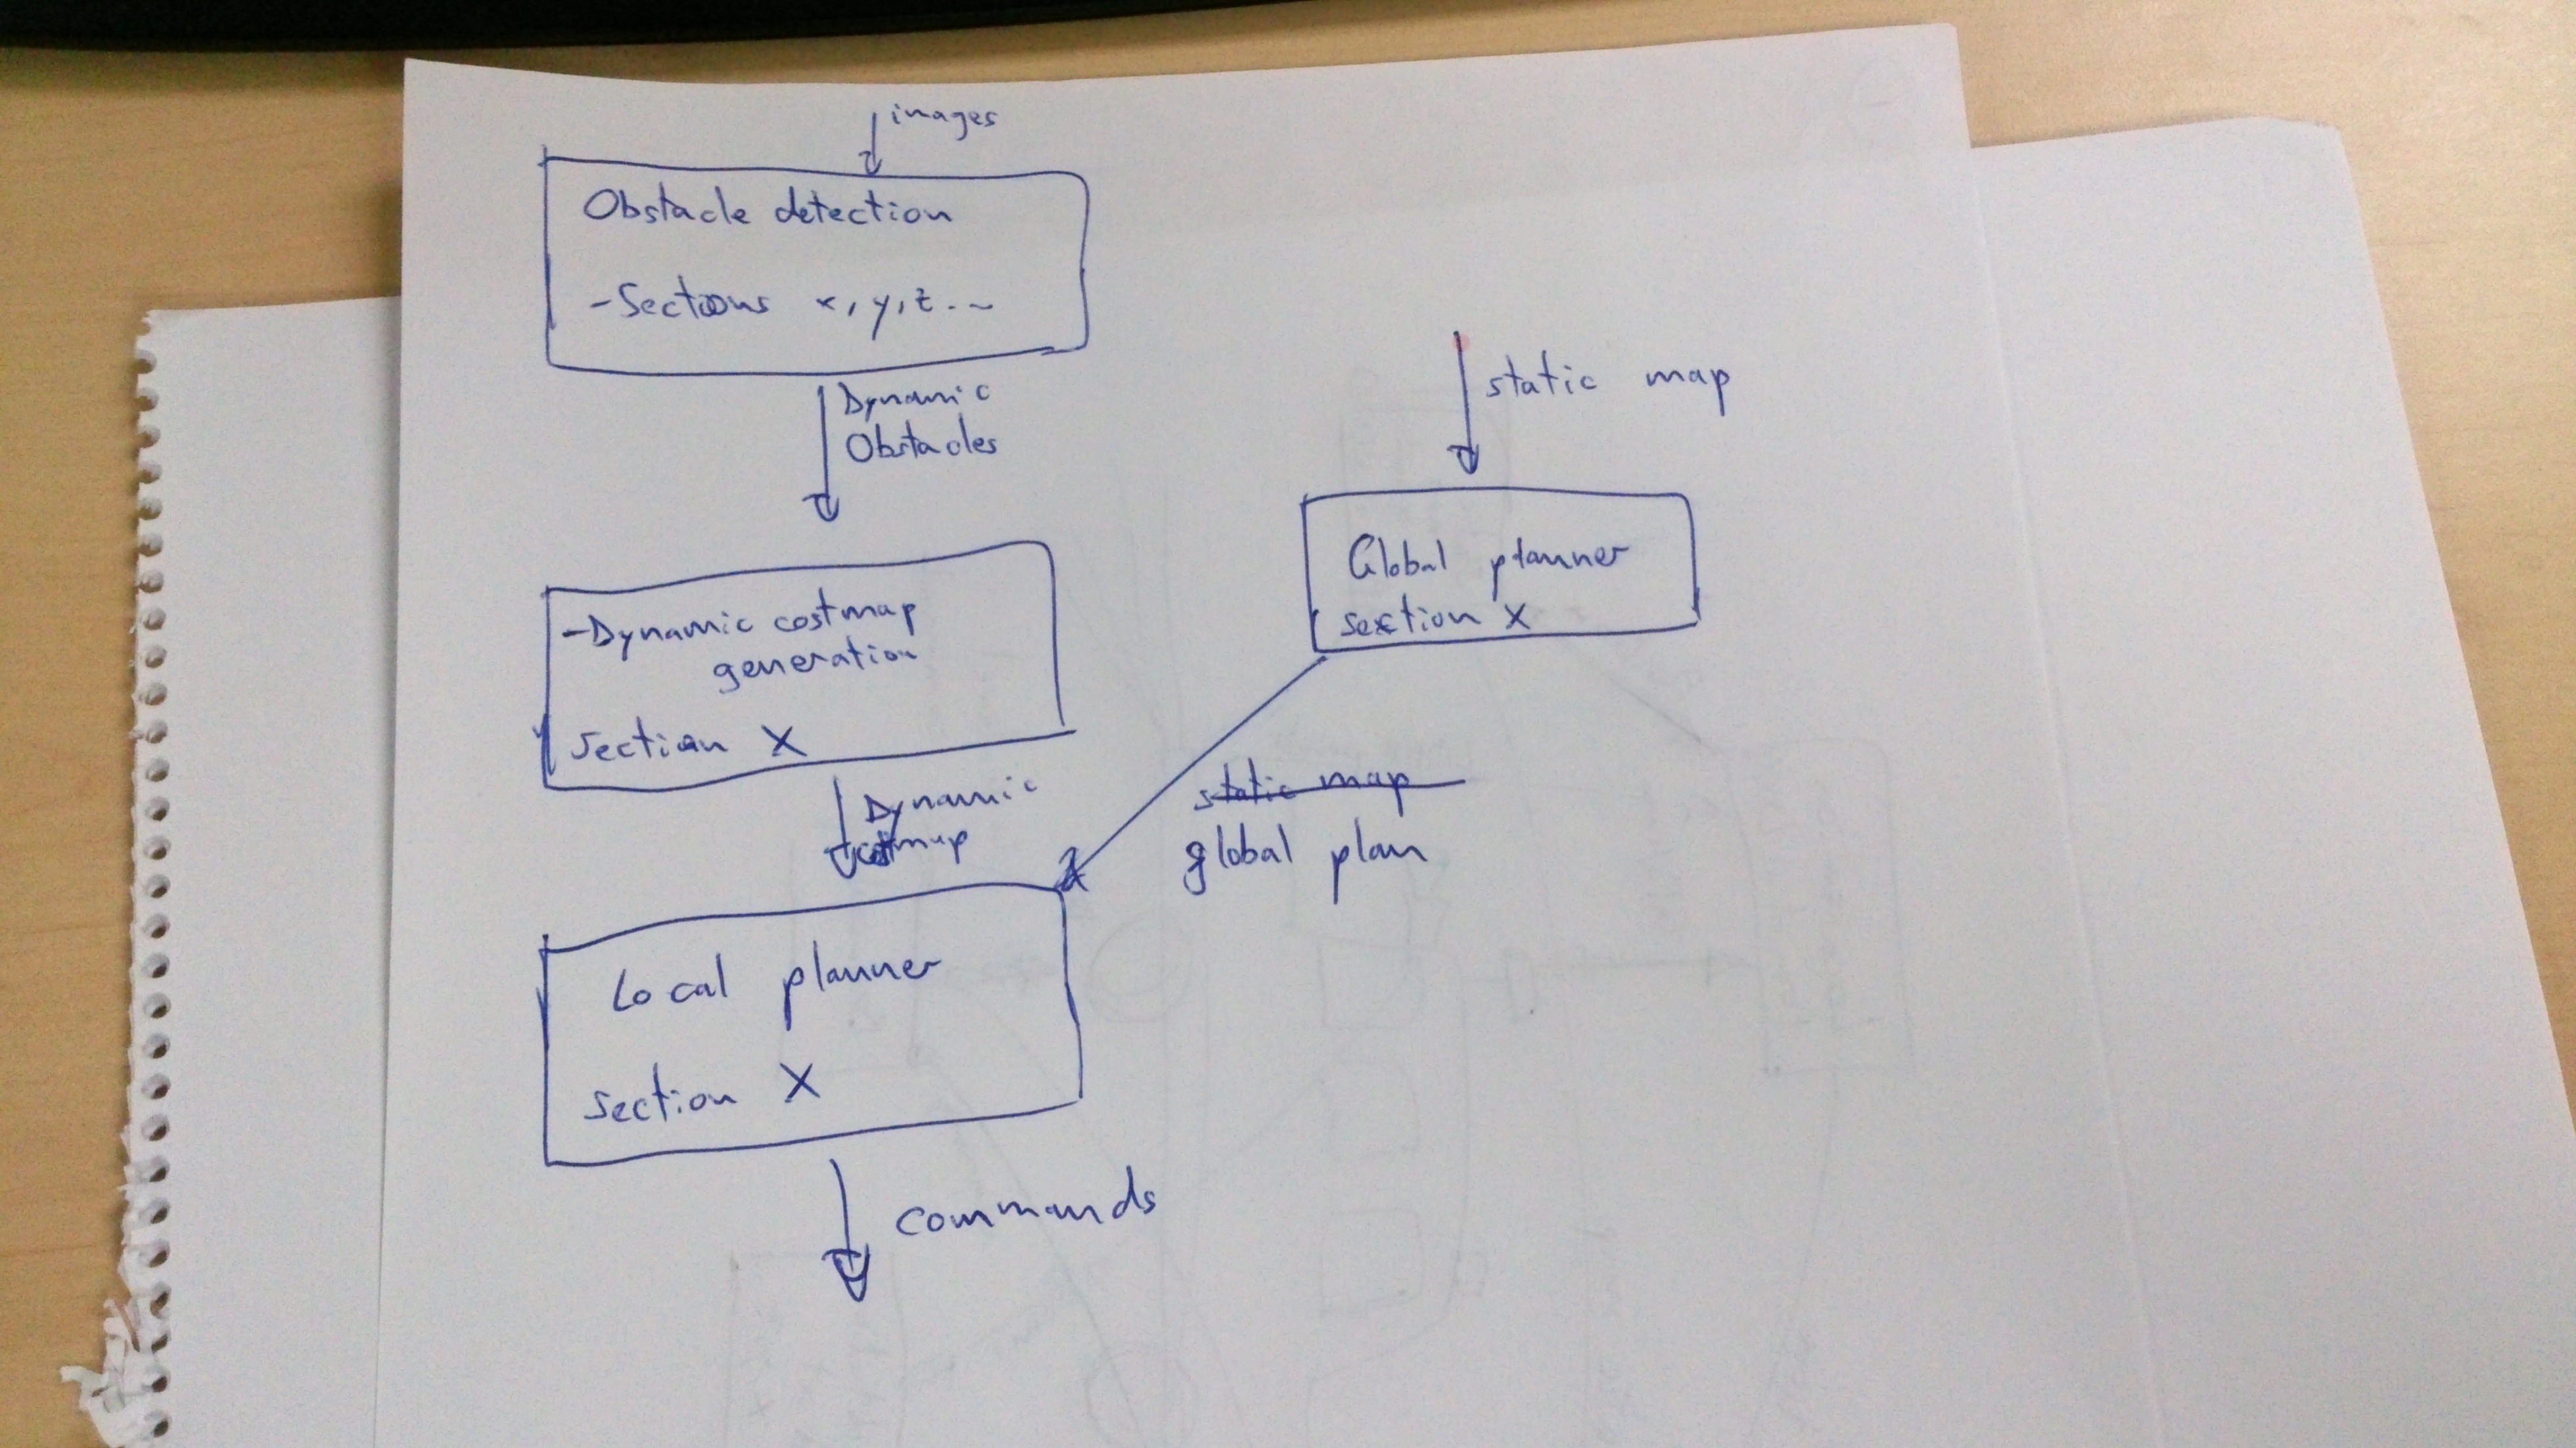
\includegraphics{pipeline}
  \caption{Pipeline of the modules described in this Thesis.}
\end{figure}

From the images captured in real-time, obstacles are located and passed to the module in charge of the generation of the dynamic costmap. At the same time, the static map is used for the generation of a feasible trajectory. Using the current position and vehicle status, the local planner tries to compute the proper commands in order to follow the global plan while trying to avoid the obstacles included in the dynamic costmap.

\section{Previous Work}\label{ch:chapter00_02}

Research on autonomous vehicles is a task being developed for a long time and for which a big effort has been carried on. A proof of that is the extensive literature existing about that topic, in special since the first of the DARPA Challenges (\cite{Buehler2007, Buehler2009}). Since then, the literature related to the topic has increased. Also, the interest on the use of Computer Vision in autonomous vehicles is growing, due to the possibilities that images offer when compared to other sensors, like \acp{LIDAR}.
In 1996, the ARGO project... \todo{Continuar desde aquí, una vez tenga una especie de historia de los vehiculos autonomos, en la intro.}
\todo{TerraMax, VIAC, Braive, Annieway y cualquier otro que pille por el camino.}
As depicted from section \ref{ch:chapter00_01}, the topics described in this thesis are quite diverse, so it is fair to review the state-of-the art of each of these topics separately.

\subsection{Change detection for obstacle localization in images}\label{ch:chapter00_02_01}

As said, one of the first attempts we made in order to detect the obstacles in the surroundings of the vehicle was the use of a geo-referenced image database. This database stored the images that later were going to be compared with the current frame being captured by the on board cameras. This work was in part inspired by the method developed by \cite{primdahl2005change}. In this work, they present an approach for the analysis of the differences in a pair of images obtained from a vehicle that pass repeatedly around the same well defined area. Their goal is to detect stationary objects that could have appeared in these area without the need of static cameras. For that, they follow a similar approach to that followed by the method described in chapter \ref{ch:chapter01}, in which each image has additional information, including their $(x, y, z, roll, pitch, yaw)$ localization values. Between the current image and the stored image, they match features and compute the inverse perspective projection. Then, they define \acp{ROI}, which are translated and rotated to a common coordinate system according to the localization information retrieved. Each pair of images is compared through the subdivision of the \acp{ROI} in a grid, determining the presence of objects for each cell in the grid.

In \cite{vallespi2012prior}, they used this approach for the alignment and change detection between images, which is later passed to an object detector based on \acp{CRF}. Other related approaches followed since then, are the works by \cite{diego2011video, evangelidis2011slice, evangelidis2011efficient}. In particular, in \cite{diego2011video} they propose a method for the spatio-temporal alignment of video sequences. They believe that one possible application for that method is the detection of vehicles for \ac{ADAS}, as well as for video-surveillance tasks. Once aligned the images, they propose to look for changes and use them for the detection of the elements that were not there in the moment of recording the original sequence, like for example a vehicle. In their work, they formulate the problem of synchronizing video sequences as the establishment of temporal correspondences between frames from the first and the second sequence. Then, all the associated frames are spatially registered.

\subsection{Non-rigid contour tracking}\label{ch:chapter00_02_02}

Based on the fact that our prototype is intended to work in a closed, well-defined area, we proposed a new technique for obstacle detection which allows the detection but also the tracking of the obstacles by the use of the static video surveillance cameras installed around the testing area. In this sense, we proposed to track not just each obstacle as a whole, but considering each part of these obstacles independently. So we are not tracking just obstacles, we are tracking their motion field in order to have full information of their movement. The advantages of this is using the output of this method also for action recognition in video surveillance applications or \ac{HMI}.

If we look at the literature, there are a lot of works on how to recover motion fields using photometric information. Many of these works are based on the information extracted from stereo  pairs or RGB-D cameras. Using the information from these sensors, some methods estimate the full 3D motion fields in order to estimate the scene flow. This is the case, for example, of the work presented by \cite{vedula1999three}. Other methods employ a stereo or a multi-view camera system to jointly estimate the motion and the geometry of the scene (in some cases under a known scene structure). Since optical flow is an approximation of the projection of the 3D motion field on the camera image plane, an intuitive way to compute scene flow is to reconstruct it from the optical flow measured in a multi-view camera system, as proposed by \cite{vedula2005three}, in which disparity information is used, or in combination with disparity estimation as \cite{huguet2007variational, li2008multi, zhang20013d}. Also, temporal consistency can be enforced (\cite{rabe2010dense}). In the case of multiple image streams, both structure and motion can be estimated in a combined way (\cite{pons2007multi, basha2013multi}). The relation of optical flow to 2D deformation capture was made clear by \cite{hilsmann2007deformable}. They utilize flow and distance constraints to recover for deformable 2D mesh from 2D images. In \cite{salzmann2007surface}, they represent a deformable surface as a triangulated surface parameterized in terms of its vertex coordinates. By doing this, they get a low-dimensional model whose dimension is independent of that of the meshes used to create it, but still captures the main deformation modes. Dimensionality reduction is done through \ac{PCA}. In \cite{wang2010monocular}, surface is also represented as a 3D triangulated mesh, but the reconstruction problem is formulated as a sequence of Linear Programming (LP) problems. Finally, in \cite{delbue2007nonrigid}, a non-linear optimization scheme is used for the estimation of the structre. Their main contribution is the development of an algorithm based on \emph{ranklets}.

About RGB-D methods, we find the method developed by \cite{quiroga2014local}. Using this sensor, they computed a local scene flow by tracking in a Lucas-Kanade framework. In \cite{spies2000dense}, they took the well studied method of \cite{horn1981determining} and extended it to RGB-D surface capture based on range flow. Then, in \cite{petit2011surface, letouzey2011scene}, geometric information from depth maps is combined with intensity variations in color images in order to estimate smooth and dense 3D motion fields. However, their approach relies on flow constraining points, which require the successful extraction of SIFT features in a deforming sequence. In \cite{birdal2012monocular}, this condition is avoided by extending the work in \cite{spies2000dense}. 

As seen, most of the recent works are based on 3D information, which requires an specific sensor as a calibrated or RGB-D camera. The application described in chapter \ref{ch:chapter02} is based on the assumption of which we will have a set of cameras installed around an specific area. Covering a big extension with those sensors will be impracticable. Moreover, most of RGB-D sensors do not work properly outdoors.

About monocular cameras, early works in this domain consider 2D motion fields between consecutive images and estimate them as the optical flow (\cite{birchfield1997derivation}). More recently, in \cite{brox2011large}, they estimate a dense optical flow field with a high accuracy in order to allow motion analysis. Also, in \cite{wang2013dense}, they show a video representation based on dense trajectories and motion boundary descriptors.

All of the named methods are based on illumination information, usually based on optical flow. In the approach proposed in chapter \ref{ch:chapter02}, we combine the use of foreground extraction methods with non-rigid point set registration techniques. In this way, we perform the tracking using just geometrical information, avoiding the dense optical flow methods described in \cite{brox2011large, wang2013dense} for monocular cameras. In our tests, we show that it is possible. We think that in the future, this geometrical information could be combined with visual information for better tracking results.

\subsection{Evaluation of stereo 3D reconstruction algorithms}\label{ch:chapter00_02_03}

At this point, all the methods presented are based on 2D information. The main problem with this is obvious: we do not know the location of the obstacles in real world coordinates. In this sense, we analyzed the behavior of some of the most used algorithms for stereo reconstruction, as well as the influence of some pre- and post-processing filters. For that, we developed a set of tools in order to perform an automatized evaluation of such methods in long sequences and with several weather conditions. 

According to \cite{Morales2012}, evaluation of stereo-analysis algorithms can be divided into two major groups: accuracy and confidence measurement methods.
In the first group, accuracy, algorithms' evaluation is performed by comparison with an available ground-truth. In this group, we find the work described in \cite{Steingrube2009}, where the images used for the evaluation are generated in a laboratory with highly controlled conditions. Another example is \cite{Vaudrey2008}, where synthetic images generated in a computer are used for the evaluation. The most remarkable work developed in this group is the one described in \cite{Geiger2012}. In this work, they generated the ground truth for about 200 scenes taken in urban and country using the information given by a \ac{LIDAR}. Ground truth for a given frame is obtained by registering 5 consecutive frames before and after the one selected and accumulating the resulting point clouds; ambiguous regions such as windows and fences are manually removed, and finally the corresponding 
disparity map is computed using calibration information. As described next, this dataset is used to validate the results obtained by our method.
In the group of confidence measurement methods, approaches are based on datasets obtained in uncontrolled environments, without a ground-truth. That is the case of the methods described in \cite{Morales2012, Steingrube2009}. In \cite{Morales2012}, the absence of ground-truth is replaced by the creation of a virtual image generated from the disparity map obtained from a pair of cameras. This virtual image is supposed to be similar to the image obtained from a third camera and, by obtaining the Normalized Cross Correlation (NCC) of both images (the virtual image and the image from the third camera), the confidence of the method is measured. In the other hand, in \cite{Steingrube2009} the evaluation system is performed at three different levels: low level, which is achieved by detecting the false stereo correspondences; mid-level, which is achieved comparing the free space in front of a car obtained with the evaluated stereo algorithm to that obtained with a LIDAR; and high-level, which is performed by 
detecting a car in front of the camera using the stereo algorithm and comparing them with the ground-truth generated using a LIDAR. The advantage of the methods in this group is that the datasets are obtained in uncontrolled environments, giving a better idea of the behavior of the methods in conditions that were not thought when experiments were done or that cannot be reproduced in a lab. Some of these methods, with some variants, have been used in our work to perform the evaluations.

\subsection{Stixel World}\label{ch:chapter00_02_04}

Apart from dense reconstruction algorithms, there are some methods that based on a stereo pair, are able to do a simplified reconstruction of the world. This reconstruction methods reject an important quantity of the information contained in the images, using just the information required for the avoidance of the obstacles. By doing so, a lot of computation time is saved. An example of this kind of algorithms is the work by \cite{badino2009stixel}, in which the world is represented through a set of ground-based vertical entities called stixels. The reconstruction of the stixels is based on the detection of the ground plane, and the stixels are grown from its basis up to the top of the detected obstacle. This allows avoiding the processing of the area of an image corresponding to the background. 
Based on this idea, some approaches have been taken. There are two main trends in the way in which stixels are computed. The main difference between them is the way in which the free space is computed. In \cite{pfeiffer2011towards, pfeiffer2013exploiting, pfeiffer2010efficient, muffert2012may}, this freespace computation is based on a disparity map and a probabilistic scheme is used in order to reduce the number of parameters. In they work, they assume that the number of objects captured along every column is small, there are not flying objects and the upper objects have a higher depths than the lower ones. In \cite{pfeiffer2013exploiting}, they improve the work presented in \cite{pfeiffer2011towards} by the use of three different stereo confidences, which are compared. In \cite{pfeiffer2010efficient}, they include a freespace computation scheme able to reduce the computational costs obtained for the previous works. They do a simple tracking and clustering of the stixels based on Kalman filters. Also, in \cite{muffert2012may} they compute the probabilities of a colission in a roundabout. There, the clustering is based on DBSCAN (\cite{ester1996density}) and freespace computation is based on a disparity map combined with B-splines \cite{wedel2009b}. 

The other research line based on stixels is based on the computation of the freespace without the need of disparity maps. It is the idea followed in \cite{benenson2011stixels, benenson2012pedestrian, benenson2012fast, gunyel2012stixels}, in which a very high frame rate is achieved by using a \ac{SAD} cube, with a value for each row, column and disparity combination. From this cube, the \emph{v}-disparity is computed and a model for the ground plane is obtained. Using the points in the boundary of the ground (obtained as a \ac{DP} problem), stixels are computed taking into account the height limitations of the expected obstacles and left-to-right occlusion constraints. 

\notsure{In section \todoref{XXX}, we introduce a method for the tracking of the stixels based on \cite{gunyel2012stixels}, in which we do the tracking of the stixels using bipartite graphs instead of \ac{DP}, as well as other metrics different from \ac{SAD}, obtaining better results both in terms of computation time and performance.}

\subsection{3D object tracking}\label{ch:chapter00_02_05}

By processing the data captured by sensors, it is desired to obtain the position, speed and size of an obstacle. However, usually sensors don't provide this information, so we need to process the information over time and do the tracking of detected obstacles. Many approaches that try to solve this problem, like \cite{danescu2012particle}, assume that obstacles have an standard geometry, and they are modeled as cuboids with associated position, size and speed vectors. This assumption is mostly correct in environments like highways, country roads, and certain urban scenarios, in which almost all the obstacles are cars, trucks or buses which can be simplified as cuboids. Also, these approaches tend to consider a flat ground.
However, this assumption cannot always done, as happens in pedestrian areas, intersections, off-road... In this case, we need to deal with specific shapes, sometimes with concave surfaces. The problem with this kind of obstacles is that methods that assume cuboid-shaped objects tend to wrap the obstacles with a convex shape, which causes an overestimation of their volume (\cite{broggi2013}). Another problem are those objects that are not laying on the ground, as happens with hanged traffic lights, tree crowns, lamps, etc. Usually, they are integrated into an occupancy grid as if they were touching the ground. About the ground plane assumption, in cases like that of an off-road scenario, it is important to estimate the real slope of the road in order to get good results.
Based on how much information they use, we can divide object tracking methods into two subcategories:
\begin{itemize}
 \item \emph{2.5D Solutions:} They do not make use of the complete information provided by 3D points. Instead of that, they tend to use elevation maps composed of uniform size cells. Each cell just stores occupancy and height information. This is the kind of methods that, as described before, usually consider obstacles as being in contact with a flat ground.
 In these methods, tracking is done before the complete reconstruction is done, in an intermediate point based on an specific feature. Based on this intermediate feature, we can distinguishing different kind of approaches:
  \begin{enumerate}
   \item \emph{Use of the 3D point as feature.} An example of this is the so called 6D vision (\cite{franke20056d}), in which the 3D stereo vision extracted information is combined with an efficient implementation of an optical flow in the image space based on a \ac{GPU}. Relevant points are tracked using a Kalman filter.
   \item \emph{Dynamic stixels.} This approach has been longer discussed in section \ref{ch:chapter00_02_04}. The 3D-situation is represented by a set of rectangular sticks named \emph{stixels}. Each stixel is defined by its 3D position relative to the camera and stands vertically on the ground, having a certain height.
   \item \emph{Tracked image features.} As example, check the work by \cite{barth2009estimating}. In this work, obstacles are represented as a rigid 3D point set which are tracked in terms of feature displacements and depth measurements.
   \item \emph{Sensor fusion.} \cite{wu2009collision} reconstruct the objects as cuboids from a stereo point cloud. In this process, position and speed values are improved to a very accurate value by the use of a radar along with stereo.
   \item \emph{Occupancy grids.} This is a very popular choice for tracking. An occupancy grid is a probabilistic map of the driving environment, which encodes the past and present knowledge from sensor data, and which can be updated dynamically when new information is available. These occupancy grids can be cartesian, with rectangular cells, polar, or even a relation between columns in an image an the disparity. An example of this is the method by \cite{danescu2012particle}, which has inspired part of the work described in section \todo { \ref{XXX}}.
   Another advantage of the model based on an occupancy grid is that it makes easier a collaborative update of the grid, which allows the usage of data from several sensors and observers.
  \end{enumerate} 
 \item \emph{3D Solutions:} Usually based on complex grid maps that use complete 3D information. Again, depending on how this grid is represented, we find 
 \begin{enumerate}
   \item \emph{Octree connected cubes.} An example is the work by \cite{wurm2010octomap} or \cite{broggi2013}.
   \item \emph{Adjacent stacks of cells}, as described in \cite{Moravec96robotspatial} 
 \end{enumerate}
\end{itemize}

\subsection{Global planning}\label{ch:chapter00_02_06}

The main goal of this thesis is the detection and avoidance of obstacles making use of the images obtained from a set of cameras mounted on a vehicle. Until now, we have seen the existing methods intended to detect objects in images, but we still do not know the existing ways for the avoidance of such objects. We consider two different levels for planning in the environment in which our testing platform will be driving. The first one, tries to get a safe and smooth trajectory that connects a certain point $A$ with a point $B$ into the map. As we are in a labyrinth-like environment, this can not be done trough a \ac{RNDF} and we have to compute that trajectory (global planner). The second level tries to follow this trajectory (local planner).
Attending to global planning, existing approaches can be classified into two big groups: classic and heuristic methods. In \cite{masehian2007classic} a compilation of some of the most relevant methods developed for each of these groups is related.
About classical methods, in general they can be considered as variations of some general approaches: Roadmap, Cell Decomposition, Potential Fields and Mathematical Programming. These methods are not mutually exclusive; in fact, a lot of approaches use combinations of them. A review of some classical methods can be checked out in \cite{hwang1992gross}.
 
About heuristic methods, these are the answer given by researchers to the limitations of the classic methods. The most representative methods inside this classification are Probabilistic Roadmaps (PRM) \cite{kavraki1996probabilistic}, Rapidly Exploring Random Trees (RRT) \cite{lavalle2000rapidly}, Level set \cite{sethian1999level}, Linguistic Geometry (LG) \cite{stilman1993network}, Simulated Annealing (SA) \cite{zhu2006robot}, Artificial Neural Network (ANN) \cite{hossain2012real}, Genetic Algorithms (GA) \cite{zhang2007evolutionary}, Particle Swarm Optimization (PSO) \cite{chen2006smooth}, Ant Colony (ACO) \cite{mou2008modified} and its variants, like the RNA algorithm described in \cite{zhu2011new}, Stigmergy \cite{cazangi2006evolutionary}, Wavelet Theory \cite{doh2005systematic}, Fuzzy Logic (FL) \cite{kladis2011energy} and Tabu Search (TS) \cite{nguyen2012multi}. For more information, the review in \cite{masehian2007classic} can be checked.

Regarding to Path Planning methods based on \ac{SVM}, several methods can be found in literature. The first one is the work presented in \cite{miura2006support}, where navigation is planned in environments in which the obstacles are known. Obstacles are randomly labeled into two classes: positive or negative. Using these two classes, a \ac{SVM} is trained and the decision boundary is used as a path. To increase the efficiency, a set of fake obstacles (guide samples) is generated at both sides of the current and the goal position, as well as in parallel to the line that joins both points (nominal line), with the objective of helping the \ac{SVM} to find a feasible path. The method works well, but it has two important limitations. The first one is that the method is highly dependent on how well fake obstacles are placed. The second one is that tentative paths are generated using different patterns (that is, some obstacles that were in the positive class are randomly labeled as negatives and vice versa) until the number of tried patterns exceeds a predetermined number and at least one feasible path is found. The consequence of using this strategy is that it is not possible to ensure that the obtained path is optimal, and the time needed to obtain at least one non-optimal path is highly dependent on the random patterns of positive/negative classes that are generated in execution time. Also, as just two classes are used, it is possible that the generated path falls too close to one of the obstacles. The original method has been optimized by the implementation described in \cite{xia2013semi}.

In \cite{sarkar2008mobile} and \cite{tennety2009support} authors divide the whole set of objects in the map into two classes and the \ac{SVM} is used to determine the maximum margin hyperplane between the data sets belonging to the two classes. Data is assigned to one or another class depending on whether the points are on the left or on the right side of the robot. After the initial labels are assigned, further classification is done using the k-nearest neighbor algorithm, with k=1. The idea is to assign to each point the label of the closest of the already labeled points. The problem of this strategy is that paths are not optimal, as it assumes that the best path is that passing along the part of each obstacle which is more clear, but it could generate zigzagging paths in environments in which a straight trajectory is possible. It does not happen in the method described in \cite{qingyang2012local}, in which a path subdivision method and a \ac{SVM} is used. They use topological maps of local environments which are extracted with little expanded nodes. Next, candidate routes are optimized using the Support Vector Machine, where the candidate routes boundary points are defined as positive and negative samples. They also extend the original \ac{SVM} \cite{cortes1995support} in order to satisfy extra constraints such as vehicle position and heading. Unlike in our contribution, in which a more extended environment is used, \cite{sarkar2008mobile, tennety2009support, qingyang2012local} are methods designed to be used in local environment maps.

One of the most important drawbacks of the method presented in \cite{miura2006support} is the need of performing a combinatorial search for the right pattern used as input for the training stage of the \ac{SVM}. A possible solution for that is using the method in \cite{yang2012safe}. In their work, a preprocessing step is used in which the Voronoi Diagram is generated using the obstacles in the map. That diagram is used to select the best path between the starting point of the robot and the goal. The path obtained using Voronoi is not smooth, so the \ac{SVM} is used to make this path smoother. The \ac{SVM} is trained using a dataset in which the sites that generated the Voronoi edges are classified as positive or negative depending on their position (left / right) regarding to the previously obtained path. The decision boundary of this \ac{SVM} will be the final path used.

As can be seen, all methods existing in the literature using \ac{SVM} for path planning purposes use just two classes. In the method presented here, there are as many classes as obstacles in the map. With our method, we try to find a new alternative to the existent \ac{SVM} based path planning algorithms. In section \ref{sec:results_comparison}, we show the advantages of using our method in comparison with other \ac{SVM} based methods.

\subsection{Local planning}\label{ch:chapter00_02_03}

With a generated path, there problem is computing the commands that the vehicle needs in order to follow that path while avoiding the occasional obstacles in the way of the vehicle. In the literature, many methods are based in searching a set of trajectories that act as intermediaries between this global path and the local path, all of them starting from the vehicle and evolving in time following an specific model, most of them following a discrete optimization scheme (\cite{thrun2006stanley, montemerlo2008junior, werling2010optimal, ferguson2008motion}).
Sampling based approaches are suitable for planning problems in the high dimensional space. The algorithm builds a collision-free path from the initial configuration to the goal path. The configuration that defines the position and orientation of the vehicle is sampled. From all the approaches of this kind, \ac{RRT} and its variants are widely used in non-holonomic motion planning applications.
\acp{RRT} are incrementally built in a way in which that the estimated distance from an specific point to the tree is quickly reduced. However, for real time implementations require efficient heuristics for the sampling configuration. 
Some examples of this kind of methods are \cite{van1997real}, \cite{lavalle2001randomized} and \cite{kuwata2009real}.

These methods compute a finite set of trajectories based on a parametric model, usually polynomial functions of a given order, The problem with this is that, despite of the fact that the space of possible solutions is reduced, allowing a efficient planning, can introduce suboptimality, reaching to overshoots or stationary offsets in curves.
Some other methods, which are inside the discrete optimization approaches, are based in the transformation of the configuration space through the Fren\'et space. Some examples are these:
\begin{itemize}
 \item In \cite{werling2010optimal}, long term objectives are performed, like speed keeping, merging, following, stopping. This is done through optimal control strategies within the Fren\'et frame of the street.
 \item In \cite{thrun2006stanley}, lateral offset is defined as the perpendicular to a established base trajectory. This allows the vehicle to drive along the road parallel to this trajectory. In order to select the optimal path, the cost function penalizes passing over obstacles and the distance respect to the center of the current road.
 \item In \cite{chu2012local}, also a set of candidate paths are generated, with endpoints in fixed positions at different offsets respect to the base frame, but they do not set this base frame in the center of the road, as it could be dangerous when computing the costs at certain scenarios. Instead of that, they use a security cost for each candidate path. Security of the path is computed by blurring the binary data of the obstacles. They also have into account certain criteria, as the smoothness cost or the path consistency between iterations.
\end{itemize}

\section{Summary}\label{ch:chapter00_03}

In this chapter, we have described a general idea of the work presented in this Thesis. Also, the pipeline of the final developed application is introduced. All this information will be explained in more detail in the following sections, including implementation details together with some results and a discussion of the advantages/disadvantages of the different methods.

